\chapter{数据预处理}
\section{数据来源}

本文所使用的基因型与表型数据主要来自于UK Biobank\cite{sudlow_uk_2015}数据库。该数据库收集并整合了2006-2010年间于英国招募的约500000名志愿者的生物样本、身体状况、功能评估、多种表型及遗传学数据。由于其所提供的丰富多样的遗传与表型信息,UK Biobank已经成为了研究多种复杂表型和遗传病的重要数据来源。本文主要基于UK Biobank的第三批发布数据开展骨关节炎相关研究。

\section{样本标注}

我们从UK Biobank数据库中获取骨关节炎患者(阳性样本)与非骨关节炎患者(阴性样本),并使用个体疾病伤害分类标准编码来对UK Biobank所提供的样本信息进行区分。国际疾病伤害及死因分类标准(The International Statistical Classification of Diseases and Related Health Problems,ICD)是由世界卫生组织所制定的根据特定规则对人群可能出现疾病进行归类的一套编码系统。\cite{who} UK Biobank已经对数据库内样本进行了ICD标注,因此我们可通过这一方法筛选研究对象。

参考其他骨关节炎的相关研究,\cite{zengini_genome-wide_2018}我们确定如下筛选规则。我们认定包含如表\ref{ICD_include}所含ICD编码的个体为骨关节炎患者。


\begin{table}[!h]
	\renewcommand{\arraystretch}{1.2}
	\centering\wuhao
	\caption{患者评判依据} \label{ICD_include} \vspace{2mm}
	\begin{tabularx}{\textwidth} { 
   >{\centering\arraybackslash}X 
   >{\centering\arraybackslash}X  }
	\toprule[1.5pt]
		ICD编码 & 分类 \\
	\midrule[1pt]
		M15-X & 骨关节炎 \\
        M16-X & 髋关节炎 \\
        M17-X & 膝关节炎 \\
        M18-X & 腕掌关节关节炎 \\
        M19-X & 其他关节炎 \\
	\bottomrule[1.5pt]
	\end{tabularx}
\end{table}
在筛选非骨关节患者时,为防止其他关节症状的干扰,我们也根据文献报道对表\ref{ICD_exclude}所含编码的个体予以排除。

\begin{table}[!h]
	\renewcommand{\arraystretch}{1.2}
	\centering\wuhao
	\caption{非患者评判依据} \label{ICD_exclude} \vspace{2mm}
	\begin{tabularx}{\textwidth} { 
   >{\centering\arraybackslash}X 
   >{\centering\arraybackslash}X }
	\toprule[1.5pt]
		ICD编码 & 分类 \\
	\midrule[1pt]
		M11-X & 软骨钙化症 \\
        M20-X、M21-X & 获得性关节畸形 \\
        M22-X & 髌骨功能异常 \\
        M23-X & 膝关节异常 \\
        M24-X & 其他关节异常 \\
        M25-X & 关节疼痛 \\
        M42-X & 脊柱软骨病 \\
	\bottomrule[1.5pt]
	\end{tabularx}
\end{table}

依照以上规则,我们从UK Biobank数据库中筛选并获得6706名骨关节炎患者作为模型训练的阳性集。同时,为保证风险预测模型训练数据的均衡性,我们又挑选出了7000名正常个体作为阴性集。两部分数据共同构成本次研究所使用的数据集。

\section{基因型位点质控}

人类基因组具有复杂性与多样性,本研究中的每个样本个体基因型数据都由数十万乃至数百万个基因型位点组成。由于目前任何算法都无法短时间内对如此多的样本进行处理,因此需要从其中选取部分具有统计学意义的位点。本文根据目前已发表的骨关节炎的GWAS结果\cite{zengini_genome-wide_2018,arcogen_consortium_identification_2019}对样本的基因型位点进行关联显著值(P-Value)与等位基因频率(Allele Frequency,AF)质控。

关联显著值是用来衡量GWAS研究中单核苷酸突变与给定性状关联显著性的一个统计量。在GWAS研究中,我们设定零假设为数据中没有SNP位点与特定性状相关联;而备择假设为至少有一个SNP位点同特定性状相关联。同时我们定义统计量$p$为当零假设为真时观察到该关联的概率。显然,$p$值越小,有越高把握在观察到关联时认为零假设为假。因此我们可以设定一个阈值,当统计量$p$低于该阈值时拒绝原假设,认为该位点同目标性状相关。\cite{chen_revisiting_2021}目前GWAS研究中对位点统计显著值的描述可通过Manhattan图
进行,Manhattan图的横坐标为SNP位点在基因组中的坐标,纵坐标为对应SNP位点在GWAS研究中的统计显著值。本研究所选区的SNP位点Manhattan图如图\ref{fig:manhattan}所示。

\begin{figure}[!ht]
\centering
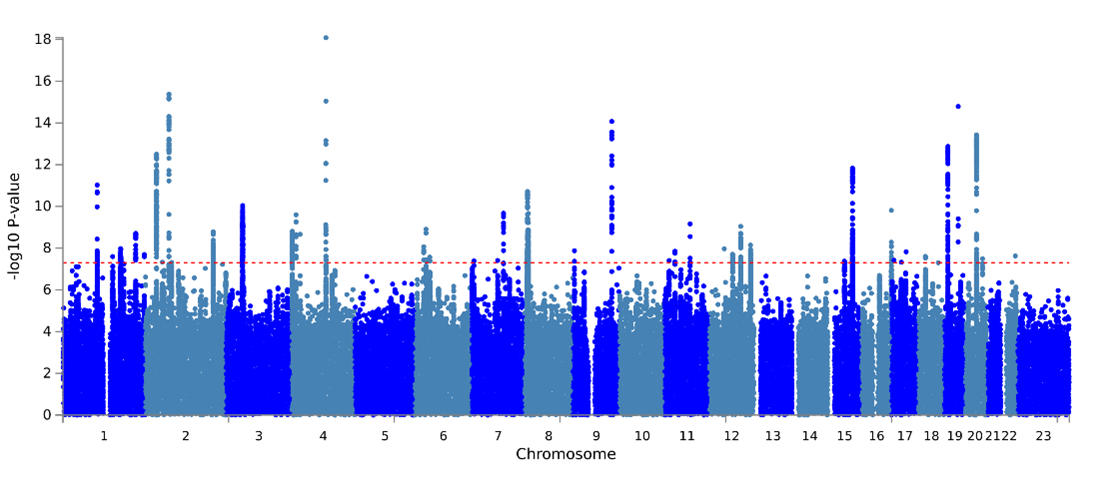
\includegraphics[width=\textwidth]{figures/Chapter2/Maha.png}
\caption{GWAS研究的Manhattan图} \label{fig:manhattan}
\end{figure}

但是,由于遗传漂变的影响,随机的基因突变也有可能具有类似相关关系。因此我们并不能认为$p$值较小的位点同目标位点直接相关,在指定阈值时需要将可能由遗传漂变所产生的位点筛去。因此我们还需要通过QQ图来完成阈值界定。QQ图是一种根据分位数对两概率分布所作的图,该图来比较两分布差别的方式。\cite{wilk_probability_1968} GWAS中的QQ图横轴为遗传漂变所产生的分布,纵轴为实际分布,当图像偏离对角线时认为这类数据并非随机漂变。因此,根据QQ图\ref{qqplot}本文确定p阈值为$10^{-5}$。

\begin{figure}[!ht]
\centering
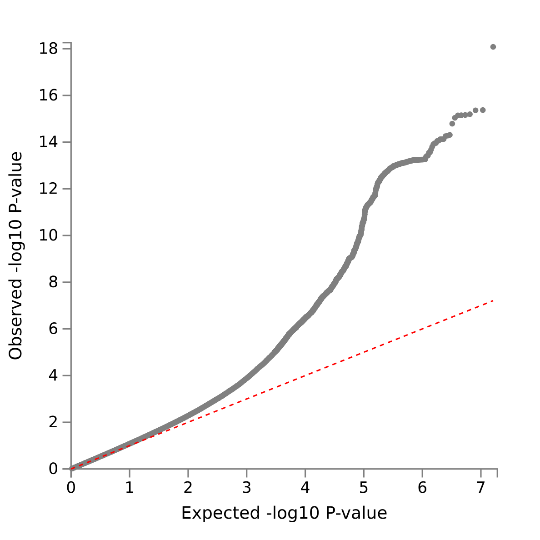
\includegraphics[width=7cm]{figures/Chapter2/qq.png}
\caption{GWAS研究的Q-Q图} \label{fig:qqplot}
\end{figure}


等位基因频率也是进行基因型数据质控时常见的评判指标。在GWAS研究中往往会发现一些出现频率很低的突变。受限于GWAS原理,大多数研究不能很好计算低等位频率位点与性状的相关性。因此在实际研究时,还需要通过等位基因频率对所得位点进行进一步质控。根据文献我们将该阈值设定为0.05\cite{marees_tutorial_2018}。

综上,本文根据关联分析显著值与等位基因频率对所得SNP位点进行筛选,最终每个个体选取选取8687个SNP位点作为待分类基因型位点。同时,我们根据位点目标突变的出现频率对数据进行编码,将基因型信息转化为算法可直接读取的数值信息。

\section{特征筛选}
目前我们已经从UKB数据库中选取了6706位骨关节炎患者作为阳性样本,每个患者包括8687个基因型特征。考虑到特征数大于样本数,可能对预测模型的准确率产生不利影响。\cite{janes_optimal_2005}本文还使用卡方法与支持向量机法对现有数据进行了特征筛选
\subsection{基于卡方的特征筛选}

卡方法使用统计学方法对输入特征与样本标注的关联进行计算,并根据计算结果筛选与样本标注相关程度较高的特征。其具体过程如下:

\begin{enumerate}
\item
  确定零假设与备择假设:对于特征与样本标注
  ,定义零假设$H_0$为该特征与样本标注无关;定义备择假设$H_1$为该特征与样本特征相关
\item
  计算特征卡方值:根据公式计算特征与样本标注的卡方值
    \begin{equation}
        \chi_c^2=\sum \frac{(O_{i}-E_i)^2}{E_i}
    \end{equation}
  其中:

  \begin{itemize}
  \item
    \(c\) 为该卡方分布的自由度
  \item
    \(O\) 为观测值
  \item
    \(E\) 为期望值
  \end{itemize}
\item
  查卡方表,拒绝或接受假设:对于计算所得卡方值,查卡方表。对照计算所得卡方值与一定自由度与置信度下的标准卡方值。当计算卡方值大于标准卡方值时接受零假设,认为该特征与样本标注无关;当计算卡方值小于标准卡方值时拒绝零假设,认为该特征与样本标注相关。基于此选择该特征
\end{enumerate}
\subsection{ 基于支持向量机的特征筛选}

支持向量机(Support Vector Machine,SVM)是一种著名的机器学习算法。其通过构建数据空间内的分类平面来实现数据分类算法。其算法核心为以下优化过程

\begin{equation}
    \min_{W,b} [C\sum_{i}max(0,1-y_i(X_i^TW+b))+l(W)]
\end{equation}

其中:

\begin{itemize}
\item
  \(X_i\) 为样本数据
\item
  \(W,b\)为超平面参数
\item
  \(y_i\)为样本标注
\item
  \(C\)为惩罚系数,即错误分类情况下对优化函数的惩罚
\item
  \(l(W)\)为超平面拟合程度的评价函数
\end{itemize}

从上式可以看出,该优化目标主要分为两部分:一部分衡量超平面对数据点的分类能力;另一部分衡量超平面对数据的拟合能力。目前常用的SVM算法中
\begin{equation}
    l(W)=\frac{1}{2}w^Tw
\end{equation}


此时该拟合函数评价分离两类数据点超平面在超空间上的距离。距离越大,证明该超平面对数据的拟合能力越好。但是,当该函数变为
\begin{equation}
    l(W)=e^T|w|
\end{equation}


此时该拟合函数又称$w$的 $l_1$范数,又称Lasso惩罚\cite{tibshirani_regression_1996},该范数可以用来评价特征在整体分类效果中的贡献\cite{fung_feature_2004}。因此本文可通过该范数对特征进行筛选。

\section{数据集描述}
经过以上步骤,我们制得包括13706位个体、每个体选取200个基因型位点的基因型数据集。数据集大小2.3GB。其中患病正样本6706例,正常负样本7000例。每个基因型位点我们通过8个字段描述,字段及其含义见表\ref{SNP_traits}。

\begin{table}[!h]
	\renewcommand{\arraystretch}{1.2}
	\centering\wuhao
	\caption{基因型位点字段信息} \label{SNP_traits} \vspace{2mm}
	\begin{tabularx}{\textwidth} { 
   >{\centering\arraybackslash}X 
   >{\centering\arraybackslash}X }
	\toprule[1.5pt]
		字段 & 含义                \\
	\midrule[1pt]
		RSID              & SNP ID            \\
    Chromosome        & SNP所在染色体          \\
    BP                & 以GRCh37为参考的碱基对位置  \\
    Effect Allele     & 与表型相关的效应等位位点        \\
    Non-Effect Allele & 与表型无关的等位位点        \\
    Beta              & 效应值               \\
    P                 & 统计显著性             \\
    MAF               & 等位基因频率           \\
	\bottomrule[1.5pt]
	\end{tabularx}
\end{table}

同时为了计算与处理方便,我们对患者基因型位点SNP数据根据效应等位位点$E$与非效应等位位点$N$进行编码,编码方式见表\ref{SNP_encoding}

\begin{table}[!h]
	\renewcommand{\arraystretch}{1.2}
	\centering\wuhao
	\caption{基因型位点编码方式} \label{SNP_encoding} \vspace{2mm}
	\begin{tabularx}{\textwidth} { 
   >{\centering\arraybackslash}X 
   >{\centering\arraybackslash}X }
	\toprule[1.5pt]
		SNP信息 & 编码\\
	\midrule[1pt]
	    $EE$ & (1,1) \\
	    $EN$ & (1,0) \\
	    $NN$ & (0,0) \\
	\bottomrule[1.5pt]
	\end{tabularx}
\end{table}

\section{本章小结}
本章介绍了本文所使用数据集获取与预处理过程。首先,根据ICD编码我们从UKB数据库中选取了6706名患病个体(阳性集)与7000名非骨关节炎个体(阴性集)作为研究对象。其次,根据关联分析显著性及基因频率从已发表的骨关节炎GWAS中筛选出感兴趣的位点并获取研究样本相应的基因型数据,之后再根据位点信息对其进行编码。最后,为了进一步减少无关的样本特征,加快计算速度,本文通过卡方法与支持向量机法对数据进行特征筛选。最终完成了由每个样本包含200个基因型信息位点的13706样本所构成的骨关节炎风险预测模型基因型数据集的构建。